% Drawing 148/02-16 -- folder 148, batch 02, archive page 34 (PDF page 35).
% Transcription: à gauche, deux sphères l'une sous l'autre : la première à cinq points sur l'équateur (trois à l'avant, dont $P$, deux à l'arrière) ; la seconde avec un tétraèdre inscrit, ses sommets marqués, et le point $P$ sur le côté.
% Kind: sphere with five points on the equator; sphere with an inscribed tetrahedron. Method 2 (schematic redraw from the facsimile). Status: partial.
% Notes: Pencil and ink. First sphere: outline, equator (front solid, back dashed), three dots on the front arc with P written under the middle one, two dots on the back. Second sphere (figure 2): outline doubled on the left; inside, a tetrahedron with a top vertex, two base vertices and an inner vertex joined to the three others, the base edge dashed; a dot labelled P to the right of the inner vertex and joined to it. Every edge is drawn between the same points. Still differs: in the second sphere the faint strokes around the inner vertex are simplified and the dots along the left edge of the tetrahedron are reduced to two. Redrawn 2026-11-12 (issue 128): to check again.
% Coordinates: 1 unit = 1 mm = 1/100 of the crop width, y downwards as on the crop (bbox in page fractions: [0.12, 0.555, 0.37, 0.74]).
% Redrawn by Claude (claude-fable-5-2), issue #128, 2026-11-12; not checked by a human; not compiled (no TeX in the session).
% Rights: reproduces part of the work -- behind RENDER_TRANSCRIPTS, never published by itself.
\documentclass[tikz,border=3pt]{standalone}
\usepackage{amsmath,amssymb}
\usetikzlibrary{patterns,arrows.meta}
\tikzset{pencil/.style={black!45}, struck/.style={black!35}, mpt/.style={circle,draw,inner sep=1.3pt}, pt/.style={circle,fill,inner sep=0.9pt}, opt/.style={circle,draw,fill=white,inner sep=1.1pt}, Rd/.style={red!75!black}, Gn/.style={green!45!black}, Br/.style={brown!70!black}}
\begin{document}
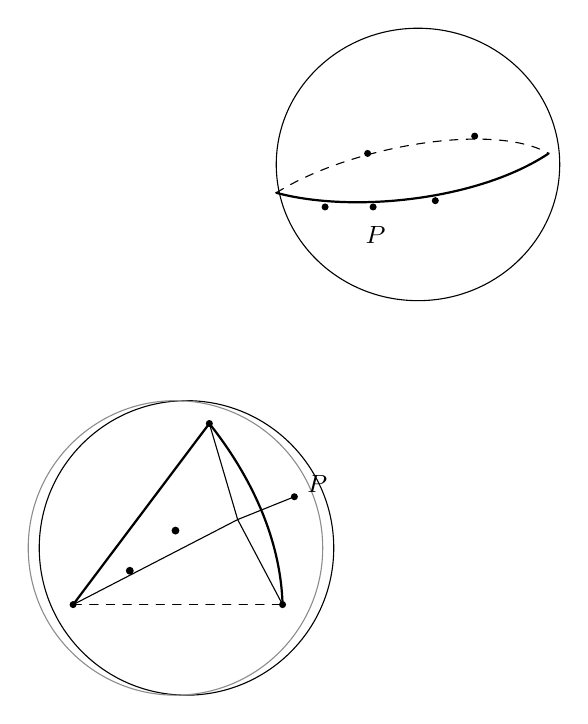
\begin{tikzpicture}[x=1mm,y=-1mm,line cap=round,line join=round,font=\small]
\draw (65.4,27.4) ellipse [x radius=18, y radius=17.3];
\draw[thick] (47.4,31) .. controls (57,33.6) and (73,32) .. (82,26);
\draw[dashed] (47.4,31) .. controls (57,25) and (75,22) .. (82,26);
\node[pt] at (53.6,32.8) {};
\node[pt] at (59.7,32.8) {};
\node[pt] at (67.6,32) {};
\node[pt] at (59,26) {};
\node[pt] at (72.6,23.8) {};
\node at (60,36.4) {$P$};
% second sphere
\draw (36,76.1) circle [radius=18.7];
\draw[pencil] (34.6,76.1) circle [radius=18.7];
\coordinate (T) at (38.9,60.3);
\coordinate (L) at (21.6,83.3);
\coordinate (R) at (48.2,83.3);
\coordinate (C) at (42.5,72.5);
\coordinate (P) at (49.7,69.6);
\draw[thick] (T) -- (L);
\draw[thick] (T) .. controls (45,68) and (48,76) .. (R);
\draw[dashed] (L) -- (R);
\draw (C) -- (T);
\draw (C) -- (L);
\draw (C) -- (R);
\draw (C) -- (P);
\node[pt] at (T) {};
\node[pt] at (L) {};
\node[pt] at (R) {};
\node[pt] at (P) {};
\fill (34.6,73.9) circle [radius=0.5];
\fill (28.8,79) circle [radius=0.5];
\node at (52.6,68) {$P$};
\end{tikzpicture}
\end{document}
